
%(BEGIN_QUESTION)
% Copyright 2011, Tony R. Kuphaldt, released under the Creative Commons Attribution License (v 1.0)
% This means you may do almost anything with this work of mine, so long as you give me proper credit

In this biogas generation system, cow manure is used as a feedstock to produce methane gas (CH$_{4}$), which is then used to fuel an engine to turn a generator and make electricity.  The waste heat from the engine is used to maintain the cascaded digesters (``reactors'' R-101 and R-102) at optimal temperatures for anaerobic bacteria to digest the manure and produce biogas (approximately 105 $^{o}$F):

$$\includegraphics[width=15.5cm]{i03486x01.eps}$$

Suppose one day there is a high-temperature engine coolant alarm indicated by TIC-43.  Determine some possible faults that could each independently account for this alarm, and also identify the first diagnostic test you would perform to troubleshoot the problem.


\underbar{file i03486}
%(END_QUESTION)





%(BEGIN_ANSWER)

Possible faults include (but are not limited to):

\begin{itemize}
\item{} TE-43 failed open
\item{} TT-43 failed with high output signal
\item{} Motor driving cooling fan lost power
\item{} Variable frequency drive for cooling fan is tripped
\item{} Fin-fan heat exchanger fins plugged with farm debris
\item{} Coolant pump motor lost power
\item{} Coolant line plugged
\end{itemize}

%(END_ANSWER)





%(BEGIN_NOTES)


\filbreak \vskip 20pt \vbox{\hrule \hbox{\strut \vrule{} {\bf Virtual Troubleshooting} \vrule} \hrule}

\noindent
{\bf Predicting the effect of a given fault:} present each of the following faults to the students, one at a time, having them comment on all the effects each fault would produce.

\begin{itemize}
\item{} 
\item{} 
\item{} 
\end{itemize}


\vskip 10pt


\noindent
{\bf Identifying possible/impossible faults:} present symptoms to the students and then have them determine whether or not a series of suggested faults could account for all the symptoms, explaining {\it why} or {\it why not} for each proposed fault:

\begin{itemize}
\item{} Symptom: {\it TIC-41 remains below setpoint for a long time}
\item{} Engine off -- {\bf Yes}
\item{} Fouled exchanger E-45 -- {\bf Yes}
\item{} TT-41 zero-shift -- {\bf No}
\item{} R-101 pump worn -- {\bf No}
\item{} TIC-48 incorrect setpoint -- {\bf No}
\item{} TIC-41 in manual mode -- {\bf Yes}
\item{} TIC-43 incorrect setpoint -- {\bf Yes}
\end{itemize}


\vskip 10pt


\noindent
{\bf Determining the utility of given diagnostic tests:} present symptoms to the students and then propose the following diagnostic tests one by one.  Students rate the value of each test, determining whether or not it would give useful information (i.e. tell us something we don't already know).  Students determine what different results for each test would indicate about the fault, if anything:

\begin{itemize}
\item{} Symptom: {\it }
\item{}  -- {\bf Yes/No}
\item{}  -- {\bf Yes/No}
\end{itemize}


\vskip 10pt


\noindent
{\bf Diagnosing a fault based on given symptoms:} imagine the ??? fails ??? in this system (don't reveal the fault to students!).  Present the operator's observation(s) to the students, have them consider possible faults and diagnostic strategies, and then tell them the results of tests they propose based on the following symptoms, until they have properly identified the nature and location of the fault:

\begin{itemize}
\item{} Operator observation: {\it }
\item{} 
\item{} 
\end{itemize}
%INDEX% Basics, control loop troubleshooting
%INDEX% Process: anaerobic digester (manure)

%(END_NOTES)


